% REVIEW-ID: logic.ch03.lattices-and-completeness
% REVIEW-TITLE: 束と完備性
\documentclass[../main.tex]{subfiles}

\begin{document}

\section{束と完備性}

束論では，順序構造の中で和と積に対応する演算を考える。ここでいう和と積は通常の数の加法・乗法ではなく，上界のうち最小のもの，下界のうち最大のものを取り出す演算である。

\begin{sidebox}[TBred]{上界・上限，下界・下限}
  上界は「集合の全要素以上にある元」であり，複数存在し得る。上限はその上界のうち最小の元である。同様に，下界は全要素以下の元，下限は下界のうち最大の元である。「上限」は単なる大きな元ではなく，最も近い上界を意味する。
\end{sidebox}

\subsection{束における双対性}

束論では，和と積が双対的な関係にある。双対的であるとは，一方の概念を上下反転させると他方の概念が得られる，いわば鏡写しのような関係である。和は上界のうち最小のものを取り，積は下界のうち最大のものを取るため，両者は順序の向きを反転させた対応になっている。

\subsection{上界と下界}

半順序構造
\[
  \mathcal{S}
  =
  \langle M,\leq\rangle
\]
において，任意の \(m \subset M\) を考える。このとき，\(m\) の上界全体を
\[
  \Up[m]
  =
  \df
  \left\{
    u
    \mid
    \text{任意の } x \in m \text{ について } x \leq u
  \right\}
\]
と定義する。\(\Up[m]\) は Upper class，すなわち上界である。これは，\(m\) のすべての元 \(x\) よりも大きい元 \(u\) をすべて集めてできるクラスである。

同様に，\(m\) の下界全体を
\[
  \Un[m]
  =
  \df
  \left\{
    u
    \mid
    \text{任意の } x \in m \text{ について } u \leq x
  \right\}
\]
と定義する。\(\Un[m]\) は Under class，すなわち下界である。これは，\(m\) のすべての元 \(x\) よりも小さい元 \(u\) をすべて集めてできるクラスである。

\begin{sidebox}[TBred]{注意}
  定義域を固定しなければ，どの範囲の元を集めて集合を定義しているのかが曖昧になる。そのため，順序構造 \(\mathcal{S}=\langle M,\leq\rangle\) を先に固定する必要がある。
\end{sidebox}

\subsection{和}

\(m\) の和は，上界のうちで最小のものとして定義される。
\[
  y
  =
  \sum_{x \in m} x
  \quad \Leftrightarrow \quad
  y \text{ は } \Up[m] \text{ に含まれる元のうちで最小のものである}
\]
ここで重要なのは，入力に対して出力が一意に決まるものを演算という点である。したがって，上界が複数あっても，そのうち最小の元が一意に定まらなければ和は演算として定義できない。

\subsection{積}

\(m\) の積は，下界のうちで最大のものとして定義される。
\[
  y
  =
  \prod_{x \in m} x
  \quad \Leftrightarrow \quad
  y \text{ は } \Un[m] \text{ に含まれる元のうちで最大のものである}
\]
ここでは，そもそも出力が存在するかどうかが問題になる。存在し，かつ一意に定まるとき，積を演算として扱うことができる。

\subsection{最大値・最小値と完備性}

次の図のような順序構造では，ある部分集合 \(m\) に対して最大値の候補が複数存在することがある。

\begin{center}
\begin{tikzpicture}[>=Stealth]
  \node (x0) at (0,0) {\(x_0\)};
  \node (x1) at (2,0) {\(x_1\)};
  \node (x2) at (3,1.5) {\(x_2\)};
  \node (x3) at (3,-1.2) {\(x_3\)};
  \node (x4) at (5,-0.2) {\(x_4\)};
  \node (x5) at (5,-1.5) {\(x_5\)};
  \node (x6) at (7,-0.6) {\(x_6\)};
  \node (x7) at (6.7,1.8) {\(x_7\)};

  \draw[->] (x0) -- (x1);
  \draw[->] (x1) -- (x2);
  \draw[->] (x1) -- (x3);
  \draw[->] (x2) -- (x7);
  \draw[->] (x3) -- (x4);
  \draw[->] (x3) -- (x5);
  \draw[->] (x4) -- (x6);
  \draw[->] (x5) -- (x6);

  \draw[TBred, thick] (2.5,-1.9) .. controls (1.8,0.8) and (3.5,2.6) .. (6.2,2.1)
    .. controls (7.0,1.2) and (7.0,-1.5) .. (5.2,-1.9)
    .. controls (4.2,-2.1) and (3.2,-2.0) .. (2.5,-1.9);

  \node[text=TBred] at (3,2.3) {\(m\)};
\end{tikzpicture}
\end{center}

この図では，最大値という解が \(x_6,x_7\) の2つ存在する。したがって，解が一意に定まらない。また，元のあいだの関係によっては，最大値や最小値の条件が互いに矛盾する場合もある。

完備性とは，このような演算の値が常に存在することを保証する性質である。以降では，数学的に扱いやすくするために完備性を前提とする。

\begin{center}
\begin{tikzpicture}[>=Stealth, scale=0.9]
  \draw (0,0) rectangle (9,3);
  \node at (-0.2,3.2) {\(M\)};

  \node (x0) at (1,1.5) {\(x_0\)};
  \node (x1) at (2.3,2.2) {\(x_1\)};
  \node (x2) at (2.3,0.8) {\(x_2\)};
  \node (x5) at (4.2,2.2) {\(x_5\)};
  \node (x3) at (4.2,1.5) {\(x_3\)};
  \node (x4) at (4.2,0.8) {\(x_4\)};
  \node (x6) at (6,0.8) {\(x_6\)};
  \node (x7) at (7.5,1.5) {\(x_7\)};

  \draw[->] (x0) -- (x1);
  \draw[->] (x0) -- (x2);
  \draw[->] (x1) -- (x5);
  \draw[->] (x2) -- (x3);
  \draw[->] (x2) -- (x4);
  \draw[->] (x3) -- (x5);
  \draw[->] (x4) -- (x6);
  \draw[->] (x6) -- (x7);
  \draw[->] (x5) -- (x7);

  \node[text=TBred] at (0.8,0.7) {\(0\)};
  \node[text=TBred] at (0.8,0.35) {空集合};
  \node[text=TBred] at (8.0,1.2) {\(1\)};
\end{tikzpicture}
\end{center}

このように，最小元と最大元を明示的に考えることで，順序構造の端点を扱うことができる。空集合に対応する最小元を \(0\)，全体に対応する最大元を \(1\) とおくと，後に述べる完備束やブール代数の構造が定式化しやすくなる。

\begin{center}
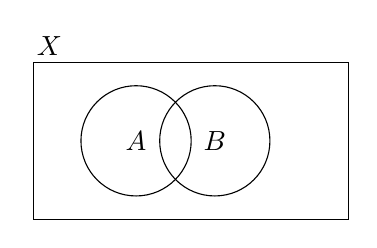
\begin{tikzpicture}
  \draw (0,0) rectangle (4,2);
  \draw (1.3,1) circle (0.7);
  \draw (2.3,1) circle (0.7);
  \node at (1.3,1) {\(A\)};
  \node at (2.3,1) {\(B\)};
  \node at (0.2,2.2) {\(X\)};
\end{tikzpicture}
\end{center}

集合演算でも，全体集合 \(X\) がなければ \(A \cup B\) や補集合を十分に定義できない。\(X\) を固定することで，集合を数学的に扱いやすい対象として整理できる。

\begin{sidebox}[TBred]{判読注意}
  元資料の「高等な？数学的な集合」付近は不鮮明である。ここでは，全体集合を固定することで集合演算を明確に扱える，という趣旨として整理した。
\end{sidebox}

\section{完備束と代数法則}

すべての部分集合について和と積が存在する束を完備束という。特に，空の部分集合に対しても和と積を定義するため，最小元 \(0\) と最大元 \(1\) が必要になる。講義ノートでは，すべての集合の部分集合に \(\varphi\) が含まれるかを考え，最小下として \(\varphi\) を設定することで完備性を確保する，という注意が付されていた。

2つの元 \(u,v\) に対する和と積は，次のように表される。
\[
  \sum_{x \in \{u,v\}} x
  =
  \df
  u+v
\]
\[
  \prod_{x \in \{u,v\}} x
  =
  \df
  u \times v
\]
この記法により，完備束は
\[
  \mathcal{S}
  =
  \left\langle
    M,\leq,\equiv,+,\times,\{0,1\}
  \right\rangle
\]
として表される。この構造において，次の代数法則が成り立つ。

\subsection{交換律}

任意の \(x,y \in M\) について，
\[
  x+y = y+x
\]
\[
  x \times y = y \times x
\]
が成り立つ。すなわち，和と積はどちらも順序を入れ替えても結果が変わらない。

\subsection{結合律}

任意の \(x,y,z \in M\) について，
\[
  (x+y)+z = x+(y+z)
\]
\[
  (x \times y) \times z = x \times (y \times z)
\]
が成り立つ。したがって，複数の元の和や積を考えるとき，括弧の付け方によって結果は変わらない。

\section{補元律・分配律・矛盾律}

\subsection{補元律}

任意の \(x \in M\) について，\(x\) と交わると \(0\) になる元を考える。すなわち，
\[
  a = -x
  \quad \Leftrightarrow \quad
  a \times x = 0
\]
となるような \(a \in M\) のうちで最大のものを，\(x\) の補元と呼び，\(-x\) と表す。

\begin{sidebox}[TBred]{注意}
  \(B\) だけでは補元として不十分である。補元は単に \(A\) と交わらない集合ではなく，全体集合 \(X\) の中で \(A\) と交わらない部分を最大限集めたものでなければならない。
\end{sidebox}

\begin{center}
\begin{tikzpicture}[scale=0.9]
  \draw (0,0) rectangle (6,3);
  \draw[TBred] (0.1,0.1) -- (0.5,0.8);
  \draw[TBred] (0.7,0.1) -- (1.2,1.0);
  \draw[TBred] (1.4,0.1) -- (2.0,1.1);
  \draw[TBred] (2.2,0.1) -- (3.0,1.4);
  \draw[TBred] (3.2,0.1) -- (4.1,1.6);
  \draw[TBred] (4.3,0.1) -- (5.4,2.0);
  \draw[TBred] (5.2,0.1) -- (5.9,1.0);
  \draw[TBred] (0.3,1.4) -- (1.1,2.6);
  \draw[TBred] (2.0,1.4) -- (2.9,2.8);
  \draw[TBred] (3.6,1.7) -- (4.7,2.9);
  \draw[TBred] (4.8,1.4) -- (5.7,2.8);

  \draw (1.2,1.5) circle (0.9);
  \draw (2.4,1.5) circle (0.9);
  \draw (4.2,1.5) circle (1.0);

  \node at (1.2,1.5) {\(A\)};
  \node at (2.4,1.5) {\(B\)};
  \node at (4.2,1.5) {\(\bar A\)};
  \node at (2.05,1.5) {\(\varphi\)};
  \node at (0.1,3.2) {\(X\)};
\end{tikzpicture}
\end{center}

集合で考えると，
\[
  A \cap B = \varnothing
\]
であっても，\(B\) が \(A\) の補集合であるとは限らない。束の記法では，
\[
  a \times x = 0
\]
であることだけではなく，そのような \(a\) のうち最大のものを取る必要がある。なお，
\[
  x \times -x = 0
\]
は補元の定義から自明である。

さらに
\[
  x + -x = 1
\]
を付け足すと，完備ブール代数の構造が得られる。

\subsection{分配律}

分配律は，和と積が互いにどのように分配されるかを述べる法則である。
\[
  x \times (y+z)
  =
  x \times y + x \times z
\]
\[
  x + (y \times z)
  =
  (x+y) \times (x+z)
\]
ここは計算で誤りやすい箇所である。結果だけでなく，どの法則をどの過程で用いたかを確認する必要がある。

\subsection{矛盾律と排中律}

命題論理では，命題 \(A\) とその否定 \(\sim A\) について，次の2つの基本法則が成り立つ。
\[
  A \land \sim A
  \quad
  \cdots
  \quad
  \text{真理値は }0
  \quad
  [\text{矛盾律}]
\]
\[
  A \lor \sim A
  \quad
  \cdots
  \quad
  \text{真理値は }1
  \quad
  [\text{排中律}]
\]
矛盾律は，命題とその否定が同時に真になることはない，という法則である。排中律は，命題またはその否定のどちらかは必ず真である，という法則である。

元資料には「偽（トートロジー）」および「倫理の世界もトートロジーにより表現する」と読める記述がある。ただしこの箇所は不鮮明である。論理学上は，常に真となる式をトートロジー，常に偽となる式を矛盾式というため，ここでは判読上の注意を残す。

\begin{sidebox}[TBred]{判読注意}
  最下部の「倫理の世界もトートロジーにより表現する」付近は不鮮明である。また，「偽」と「トートロジー」は通常の論理用語としては一致しないため，元資料の記述を注意つきで保持した。
\end{sidebox}

\end{document}
